\documentclass[crop, tikz, border=10pt]{standalone}
%\usetikzlibrary{...}% tikz package already loaded by 'tikz' option
\usetikzlibrary{matrix}
\usepackage{color}
\begin{document}
\color{yellow}
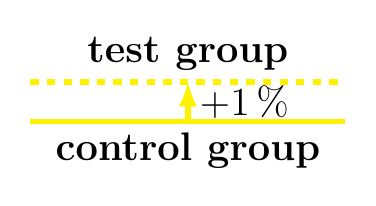
\begin{tikzpicture}[draw=yellow]
%\tikzset{circle node/.style = {circle, inner sep=1pt, draw, fill=white}}
\tikzset{edge/.style = {->,> = latex, line width=2 pt}}

\path[draw=yellow, line width=2, dashed] (0,.5) -- (4, .5) node[midway, above]{\Large \textbf{test group}};           
\path[draw=yellow, line width=2] (0,0) -- (4, 0) node[midway, below]{\Large \textbf {control group}};   
\draw[edge] (2, 0) -> (2, .5) node[midway, right]{\Large \textbf{$+1\,\%$}};   
    
\end{tikzpicture}
\end{document}